\setauthor{Marcel Pouget}
Die Arbeit wurde zusammen mit der Firma FlexSolution GmbH entwickelt. Diese stellten auch die benötigte Hardware in Form von Raspberrys, den Ladestationen und Arbeitsplätzen zur Verfügung. Bei Problemen standen zwei Mitarbeiter immer zu Verfügung und halfen mit, Probleme zu lösen. Die Basis der Arbeit wurde schon in einem Ferialpraktikum im Sommer 2021 gelegt, in welchem mit Zusammenarbeit qualifizierter Arbeiter die Ladestationen montiert wurden. Der programmierende Anteil des Projektes wurde im Zuge eines Praktikums im Jahre 2022 umgesetzt. Dieses dauerte 4 Wochen und war nur für die Entwicklung der Arbeit gedacht.

Die Idee eines Lademanagers entstand im Frühjahr 2021, als die Photovoltaikanlage der Firma fertiggestellt wurde. Marcel war zu dieser Zeit als Werksstudent bei der Firma angestellt und bekam das Angebot, dieses Projekt als Diplomarbeit umzusetzen.

\section{Herangehensweise}

Nach einem ersten Briefing mit Alfred Pimminger wurden erste Pläne für das Projekt ausgearbeitet. Vor allem der Aufbau und das Zusammenspiel mit den firmeninternen Systemen war dabei äußerst wichtig. Die erste Skizze des Projektes sah dabei wie folgt aus: 
\ref{fig:impl:ersteSkizze}

\begin{figure}[h t]
  \centering
  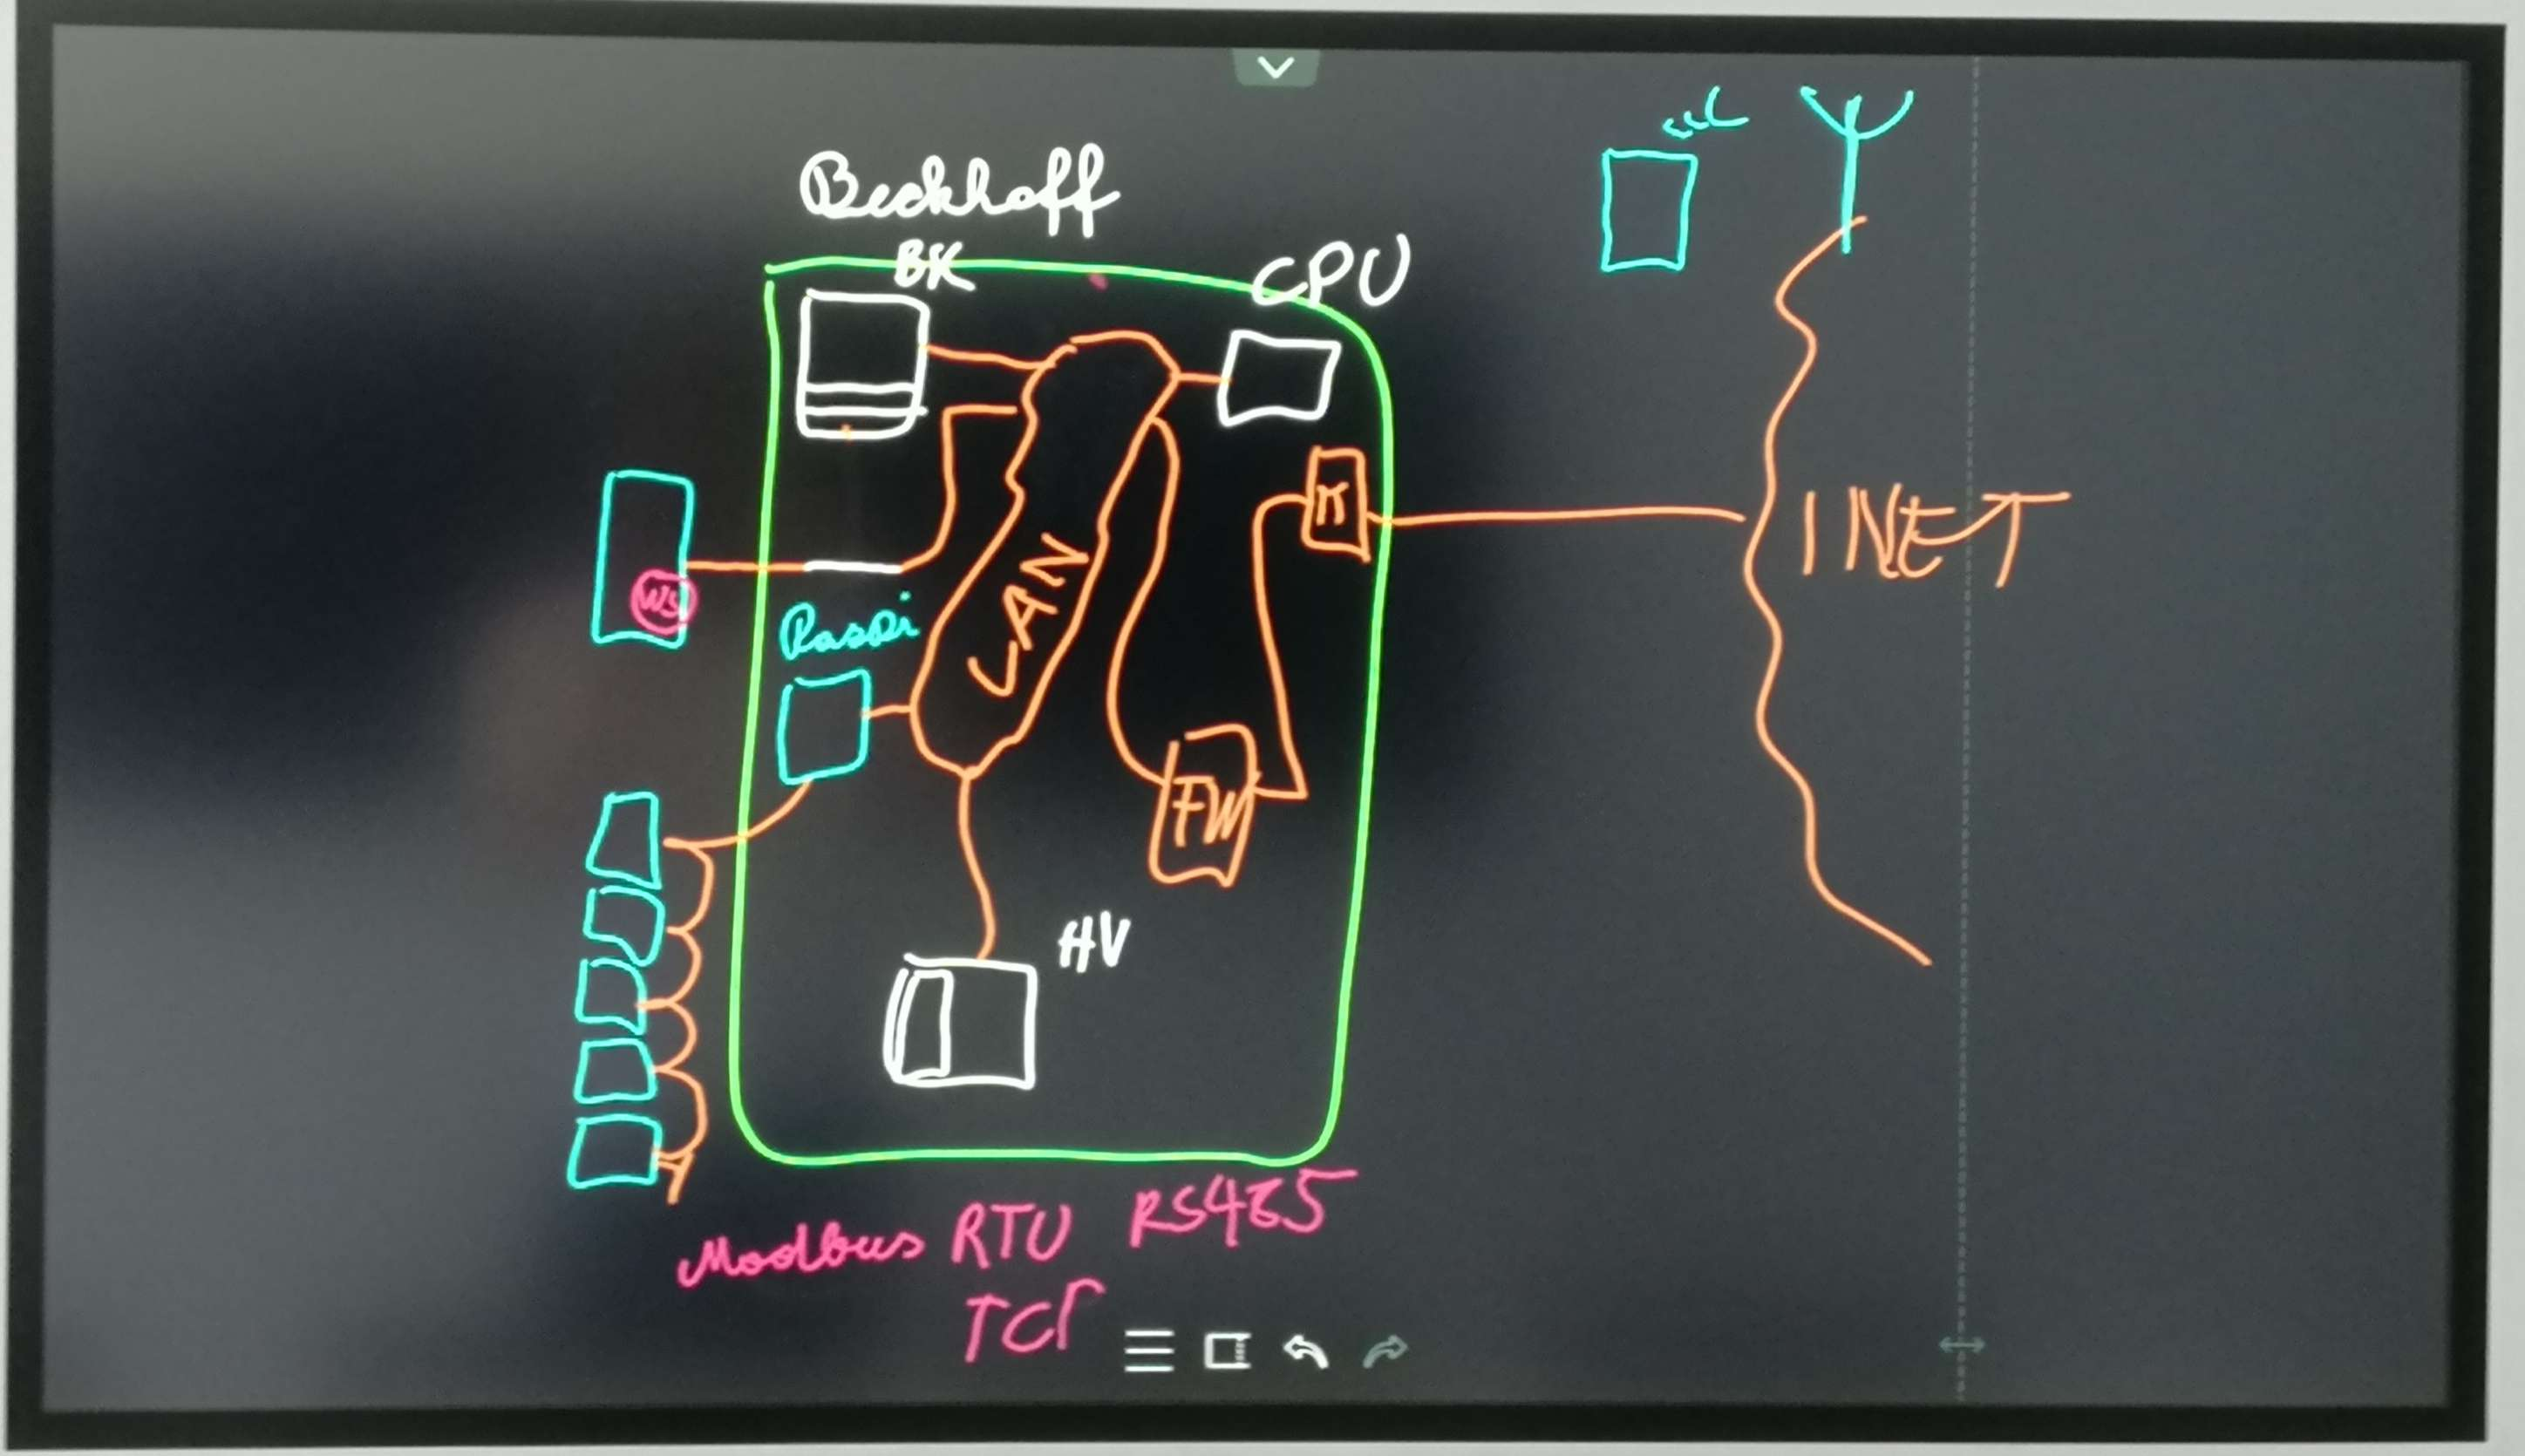
\includegraphics[scale=0.15]{pics/ersteSkizze.jpg}
  \caption{Erste Planung auf einem Whiteboard}
  \label{fig:impl:ersteSkizze}
\end{figure}
 

Der Aufbau hat sich im Laufe der Entwicklung leicht verändert, jedoch blieb die Grundbasis erhalten. Siehe \ref{section:aufbaudesProjektesFlexlogger}. Das Projekt über einen Logger entstand erst etwas später. Auch hier wurde der Aufbau der Arbeit während eines Meetings mit Alfred besprochen, jedoch geschah die Umsetzung erst einige Monate später. Hier war der Plan, von verschiedensten Flextasks die Daten zu speichern, da diese bis jetzt immer gelöscht wurden. Die Planung für den Aufbau des Projektes geschah erst im Zuge der Entwicklung, siehe \ref{AufbauDesProjektesWallbox} 
\setauthor{Marcel Pouget}
 
 
\section{Zeitplan}
\setauthor{Marcel Pouget | Teresa Holzer}
 

Um das Projekt problemlos umsetzen zu können, wurden noch vor dem eigentlichen Projektstart zehn Meilensteine angelegt.   

\begin{compactitem}
  \item 30.06.2022 Fertigstellung Pflichtenheft  
  \item 07.08.2022 Datenbank aufsetzen (Flexlogger)  
  \item 07.08.2022 Flexlogger Server aufsetzen (Flexlogger)  
  \item 07.08.2022 Task für Kommunikation mit den Wallboxen aufsetzen (Wallboxen)  
  \item 14.08.2022 Geloggte Daten kommen bei dem Frontend an (Flexlogger)  
  \item 14.08.2022 Task für das Steuern der Wallboxen aufsetzen (Wallboxen)  
  \item 21.08.2022 Daten werden visualisiert (Flexlogger)  
  \item 21.08.2022 Die Verbindung zwischen UI und den Wallboxen steht (Wallboxen)  
  \item 31.08.2022 Fertigstellung der Website für die Wallboxen (Wallboxen)  
  \item 31.08.2022 Fertigstellung des Flexloggers (Flexlogger) 
\end{compactitem}
 
\section{Verwendete Tools}
 Während der Entwicklung des Projektes wurden viele verschiedene Systeme verwendet, um den Verlauf des Projektes zu beschläunigen. Welche dieser Tools in verwendung waren, und wie sie eingesetzt wurden, wird in diesem Kapitel beschrieben.
 
 
\subsection{Latex [M]} \setauthor{Marcel Pouget}

Latex ist eine Software, welche es ermöglicht, Texte, Graphiken und Bilder zu layoutieren und zu exportieren. Sie basiert auf dem Textsatzsystem TeX und arbeitet nach der Methode WYSIWYM (What You See Is What You Mean). Das heißt, dass der Text, welcher im Endprodukt angezeigt werden soll, in einem Quelldokument erstellt wird und erst nach dem Kompelieren eine Formatierung enthält. Das ermöglicht es, schnell Verweise zu anderen Textstellen zu integrieren, eine automatische Beschriftung für Bilder und Quellen, ein Literaturverzeichnis, welches einen guten Überblick bietet. Natürlich darf ein automatisch-generiertes Inhaltsverzeichnis nicht fehlen, welches mit Verschieben der Komponenten aktualisiert werden kann. Das ermöglicht es, ganze Kapitel innerhalb von Sekunden neu zu strukturieren, ohne dass Beschriftungen oder andere Layouts ihre Gültigkeit verlieren. Ein paar weitere Vorteile von Latex sind:  

\begin{compactitem}
    \item Die Qualität der Dokumente ist sehr hoch. 
    \item Die Dokumente werden automatisch klar und einheitlich formatiert. Da dies bei wissenschaftlichen Arbeiten immer eine Voraussetzung ist, ist Latex oft die richtige Wahl. 
    \item Es können mathematische Formeln, Codebeispiele, Tabellen, Bilder und vieles mehr ohne Probleme mit der Formatierung eingebettet werden. 
    \item Die Ausgangstexte sind plain Text, das heißt, es kann sowohl von jedem gelesen, verstanden als auch bearbeitet werden. 
    \item Da größere Arbeiten immer aus mehreren Dokumenten bestehen, ist Latex sehr flexibel. Man kann die Struktur mit Ordnern beliebig wechseln, Einstellungen für eine gewisse Anzahl an Seiten oder für das ganze Dokument treffen. Dadurch eignet es sich sehr gut für Projekte, an denen mehrere Autoren gleichzeitig arbeiten.  
    \item Latex ist opensource, und sehr gut dokumentiert.  Es gibt viele Anleitungen dazu, wie man es benützt und wird von jedem gängigen Betriebssystem unterstützt. 
    \item Außerdem gibt es für verschiedene Anwendungszwecke vorgefertigte Templates, welche das Arbeiten erleichtern. In solchen gibt es schon eine globale Einstellung für Schrift, Absätze, Nummerierungen und Deckblätter. Dies erleichtert die Arbeit sehr, da man nicht immer von vorne beginnen muss, wenn man ein neues Dokument erstellen möchte.  
\end{compactitem}

Diese Punkte ermöglichen es dem Autor, sich nicht auf das Layout konzentrieren zu müssen, sondern ermöglicht es, sich nur auf den Inhalt zu fokussieren.  Der Rest wird voll und ganz von der installierten Software übernommen. 

 

Starten kann man ein Latex-Projekt in jedem Beliebigen Editor.  Wichtig dabei ist nur, dass das Programm Latex an sich auf dem Rechner installiert wurde und alle Abhängigkeiten automatisch heruntergeladen wurden. Editoren wie Visual Studio Code unterstützen eigene Plugins für Latex, in welchem das ganze Projekt übersichtlich an der Seite angezeigt wird. Dies bietet den Vorteil, dass nicht nur eine Live-Vorschau ermöglicht wird, sondern auch die Navigation in komplexen Projekten vereinfacht wird.  

  

Ein neues Projekt wird angelegt, indem eine \grq.tex\grq Datei erstellt wird. In dieser kann dann schon reiner Text geschrieben werden, jedoch wird das Layout noch nicht die gewünschte Form bekommen.    

Um das zu erreichen, gibt es die Möglichkeiten von sogenannten Templates, welche oft von Firmen, Universitäten oder Schulen angeboten werden (siehe Haslinger Template). In solchen vorgefertigten Projekten gibt es schon eine klare Struktur und Files, welche sich um das Layoutieren kümmern. Vorteil davon ist, dass sehr viel Arbeit von Latex übernommen wird und der Fokus rein auf den Inhalt gelegt werden kann. 


\subsection{Intellij [M]} \setauthor{Marcel Pouget}

Intellij ist eine IDE (Integrated Development Environment, oder zu Deutsch: Integrierte Entwicklungsumgebung), welche für die Entwicklung in Java und Kotlin optimiert ist. Das Programm bietet eine Vielzahl an Hilfsmitteln und Plugins, um das Entwickeln zu vereinfachen. Von intelligenter Code-completion bis zu intuitiven Debugging Möglichkeiten ist alles dabei.  Und sollte eine Sprache oder ein Feature nicht unterstützt werden, sind im Plugin-Store noch unzählige Anpassungen, welche die IDE noch besser machen. Ein großer Bestandteil der Software ist die Möglichkeit, Build-Tools wie Maven oder Gradle von Haus aus zu verwenden. Ein Beispiel sieht man bei \ref{fig:impl:WallboxMavenTap}. Außerdem ist es möglich, ohne Windows / Linux Umgebungsvariablen den Code direkt in der Applikation zu testen. Dafür wird die ausgewählte JDK heruntergeladen, und so konfiguriert, dass zuverlässig jeder Code mit einem Click gestartet werden kann. Sollten Dependencies fehlen, kann man sie mit einer instigierten Suche hinzufügen und mit einem eigenen Tap für Maven herunterladen. 

\begin{figure}[h t]
    \centering
    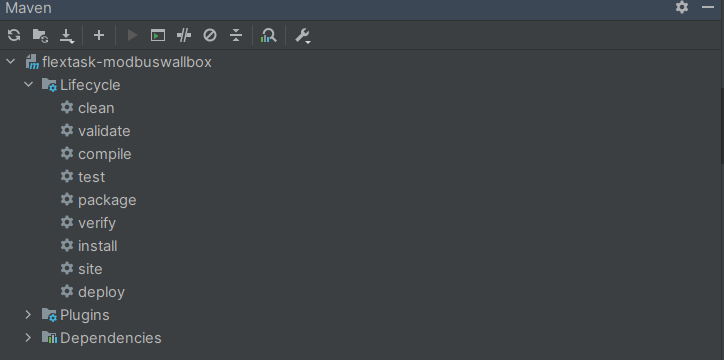
\includegraphics[scale=0.55]{pics/MavenOverfiew.png}
    \caption{So sieht der Maven-Tap in Intellij aus}
    \label{fig:impl:WallboxMavenTap}
  \end{figure}

  Die Ordnerübersicht und die Möglichkeit, Variablen in einem ganzen Projekt zu refactoren, sind unterstützend, wenn es um Änderungen in den eigenen Projekten geht. Eine globale Suche und eine Formatierungsfunktion helfen dabei, die User Experience zu erhöhen. Die Intellij IDE kann man in zwei Produkte unterteilen: die kostenlose Opensource-Kommunikation-Edition und die kostenpflichtige Ultimate-Version. Während die kostenlose Version eine gute Möglichkeit ist, schnell kleinere Programme umzusetzen, ist vor allem Ultimate besser geeignet, große Projekte mit mehreren Mitarbeitern zu bewältigen. Dafür ist selbstverständlich ein Versionscontrol-System integriert, welches sich problemlos mit Anbietern wie z.B. Github nutzen lässt.  

Und auch wenn IntelliJ IDEA in erster Linie für die Java- und Kotlin-Entwicklung vorgesehen wurde, unterstützt die IDE auch viele weitere gängige Programmiersprachen wie Groovy, Javascript, Typescript und SQL. Für letzteres gibt es sogar einen eigenen Tab, in welchem man ohne Probleme Datenbankverbindungen aufbauen und testen kann. Ein kleiner Überblick über die einzelnen Tabs und sogar eine Console für SQL-Querrys sind auch geboten.   

\begin{figure}[h t]
  \centering
  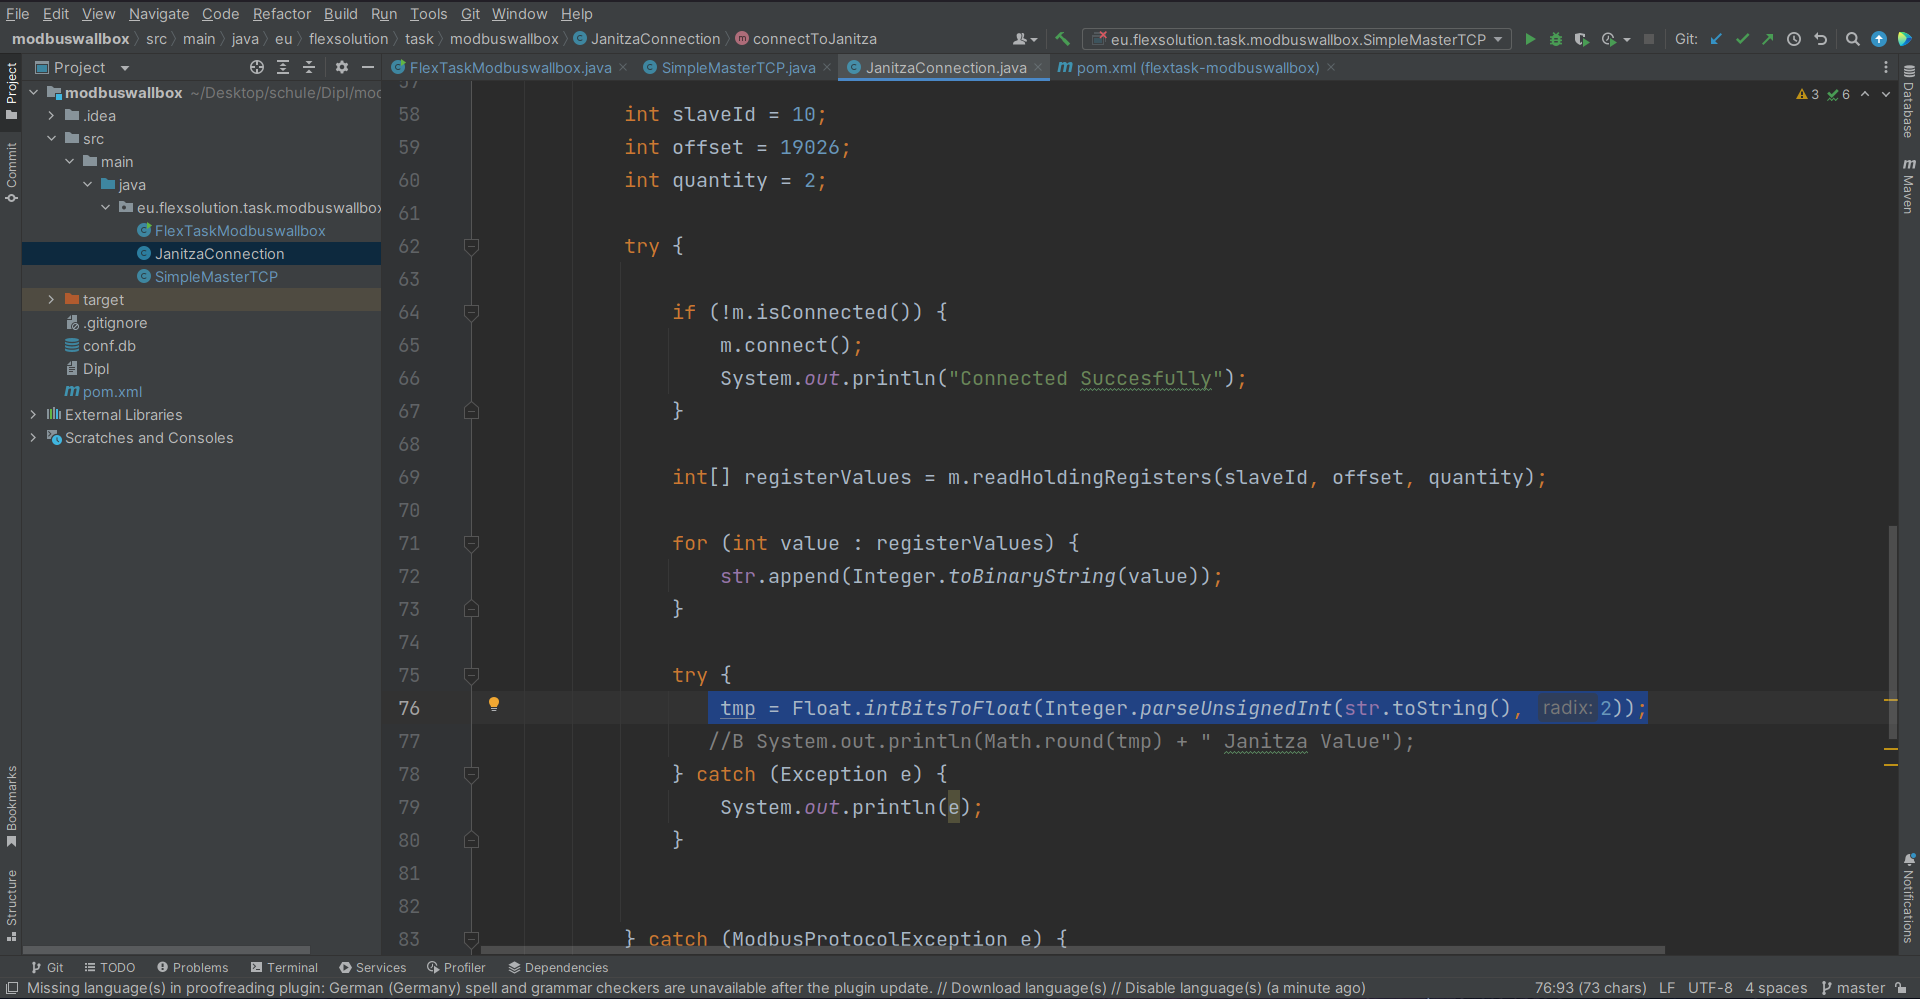
\includegraphics[scale=0.2]{pics/IntellijOverfiew.png}
  \caption{Ansicht von einem Intellij Projekt}
  \label{fig:impl:WallboxIntellij}
\end{figure}

 

\subsection{Webstorm [T]} \setauthor{Teresa Holzer}
% < https://www.jetbrains.com/de-de/webstorm/
\setauthor{Teresa Holzer [T]}\setauthor{Teresa Holzer}
WebStorm, Interface siehe Abb. \ref{fig:impl:webstorm}, wird als Entwicklungsumgebung für JavaScript und JavaScript-ähnliche Sprachen definiert. Es ist außerdem geeignet für die Entwicklung mit Angular, da ein neues Projekt direkt in WebStorm erstellt und in der Entwicklungsumgebung gestartete werden kann. WebStrom wurde, genau wie IntelliJ, von JetBrains entwickelt und liefert eine Reihe von Hilfestellungen, um JavaScript optimal programmieren zu können. WebStorm beinhaltet eine automatische Code-Überprüfung sowie die automatische Komplettierung von einzelnen Codezeilen. WebStorm beinhaltet außerdem einen bereits eingebauten Run- sowie Debug-Button, durch welchen das Starten in der Konsole wegfällt. Zusätzlich können in WebStorm verschiedenste Plugins hinzugefügt werden, welche das Erscheinungsbild verändern, andere Sprachen überprüfen können und vieles mehr. \cite{webstormOfficialSite}

\begin{figure}[h t]
    \centering
    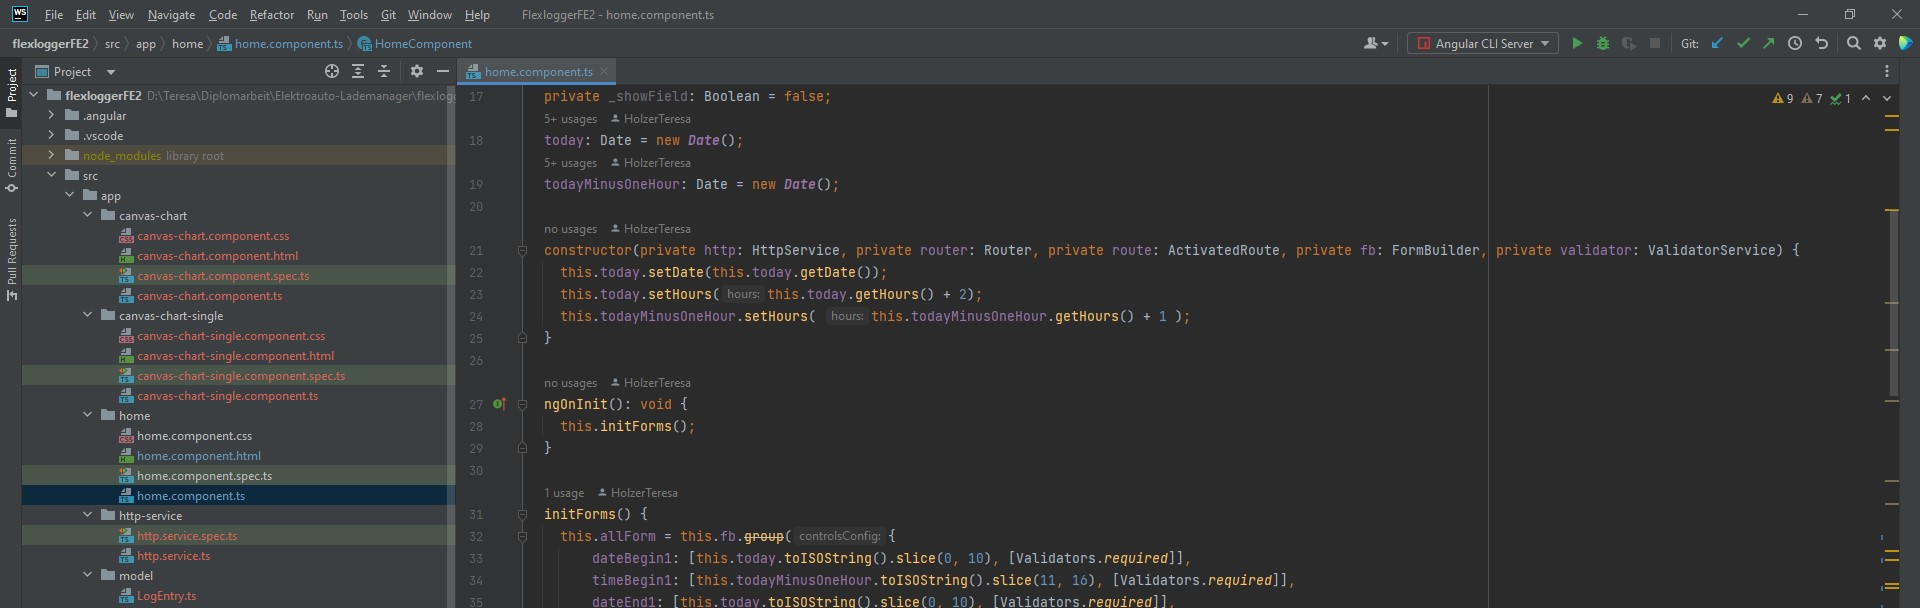
\includegraphics[scale=0.38]{pics/webstorm.jpg}
    \caption{WebStorm}
    \label{fig:impl:webstorm}
  \end{figure}


\subsection{Linux Terminal [M]} \setauthor{Marcel Pouget}
Vieles der Entwicklung fand in der Kommandozeile von Linux statt. Von der Überwachung des Status der Tasks, bis hin zum Starten der App lief alles in einem Terminal ab. Dabei handelt es sich um ein Programm, welches einen Text von einem User entgegennimmt, und als Befehl interpretiert. Dadurch lassen sich Verbindungen zu weiteren Geräten via SSH ermöglichen, um aus der Ferne Projekte zu entwickeln. So kann der Raspberry Pi4 in einem Schaltschrank der Firma montiert sein, und trotzdem kann ein Entwickler aus dem Büro die Einstellungen verändern.   

Mit einer sogenannten CLI (Command Line Interface) lassen sich Programme ohne graphische Useroberfläche bedienen, Ordner und Files verwalten, und ganze Serverstrukturen verwalten. 
\subsection{Discord [M]} \setauthor{Marcel Pouget}
Discord ist eine kostenlose App für Kommunikation via Sprache, Chat und Video. Dies ermöglicht einen schnellen, reibungslosen Austausch zwischen einzelnen Personen bis hin zu großen Gruppen. Im Zusammenhang dieser Arbeit wurde die Applikation dafür benutzt, um Aufgaben zu verteilen, Informationen auszutauschen und Meetings zu halten. Ein Server für dieses Projekt wurde erstellt, um immer einen Überblick der aktuellen Dokumente zu bekommen. Auch die Links zu Informationen, Terminen und dem Google Drive-Laufwerk wurden gespeichert.   

Discord half vor allem bei der Organisation unter den Projektmitgliedern. Dadurch konnte eine reibungslose Kommunikation gewährleistet werden  
\subsection{Google drive [T]} \setauthor{Teresa Holzer}

% < https://one.google.com/about
Google Drive ist ein Cloud-Speicher, welcher für das Online-Speichern von Google Docs, Google Tabellen, Google Präsentationen und Google Formularen verwendet werden kann. Außerdem können Bild- und andere Formate hochgeladen und somit gesichert werden. Google Drive kann kostenlos durch das Erstellen eines Google-Accounts verwendet werden. Google stellt dabei 15GB Speicher frei zur Verfügung, danach kann durch ein monatliches Abo-Modell mehr Speicherplatz erlangt werden. \cite{OneDriveOfficialSite}

Google Drive wurde im Rahmen dieser Diplomarbeit genutzt, um Dokumente und Dateien für alle Projektmitglieder leicht zugänglich zu machen.

\subsection{Visual Studio Code [T]} \setauthor{Teresa Holzer}
% < https://code.visualstudio.com/docs
Visual Studio Code, Interface siehe Abb. \ref{fig:impl:vsCode}, ist ein leistungsstarker Code Editor. Es ist verfügbar für Windows, Linux und macOS. 
Einer der größten Vorteile von VS Code ist ein eingebautes Support-Tool für JavaScript, TypeScript und Node.js. Außerdem verfügt es über zahllose Erweiterungen für andere Programmiersprachen. VS Code besitzt auch einen Run und Debug Modus, um Programme direkt in der Umgebung ausführen zu können. 
VS Code kann vielfältig eingesetzt werden und aufgrund der Erweiterungen nach Belieben personalisiert werden. \cite{VSCodeOfficialSite}

Um nur ein paar der Erweiterungen zu nennen, welche VS Code wandelbar machen: 

\begin{compactitem}
    \item Microsoft Visual Studio Live Share: Mithilfe dieser Extension ist es möglich, gleichzeitig von mehreren Computern an einem Projekt zu arbeiten.
    \item C, C++, Python, ... : Durch diese Extensions kann leichter in der jeweiligen Programmiersprache programmiert wird, da IntelliSense und debugging features hinzugefügt werden.
    \item Visual Studio Code Remote – SSH: Mittels dieser Extension kann jeder entfernter Rechner mit einem SSH-Server als Entwicklungsumgebung verwendet werden.
\end{compactitem}
\cite{VSCodeOfficialSite}

Zur einfachen Ansicht von Code sowie zum Verfassen des schriftlichen Teils der Diplomarbeit mithilfe von Latex wurde VS Code verwendet.

\begin{figure}[h t]
  \centering
  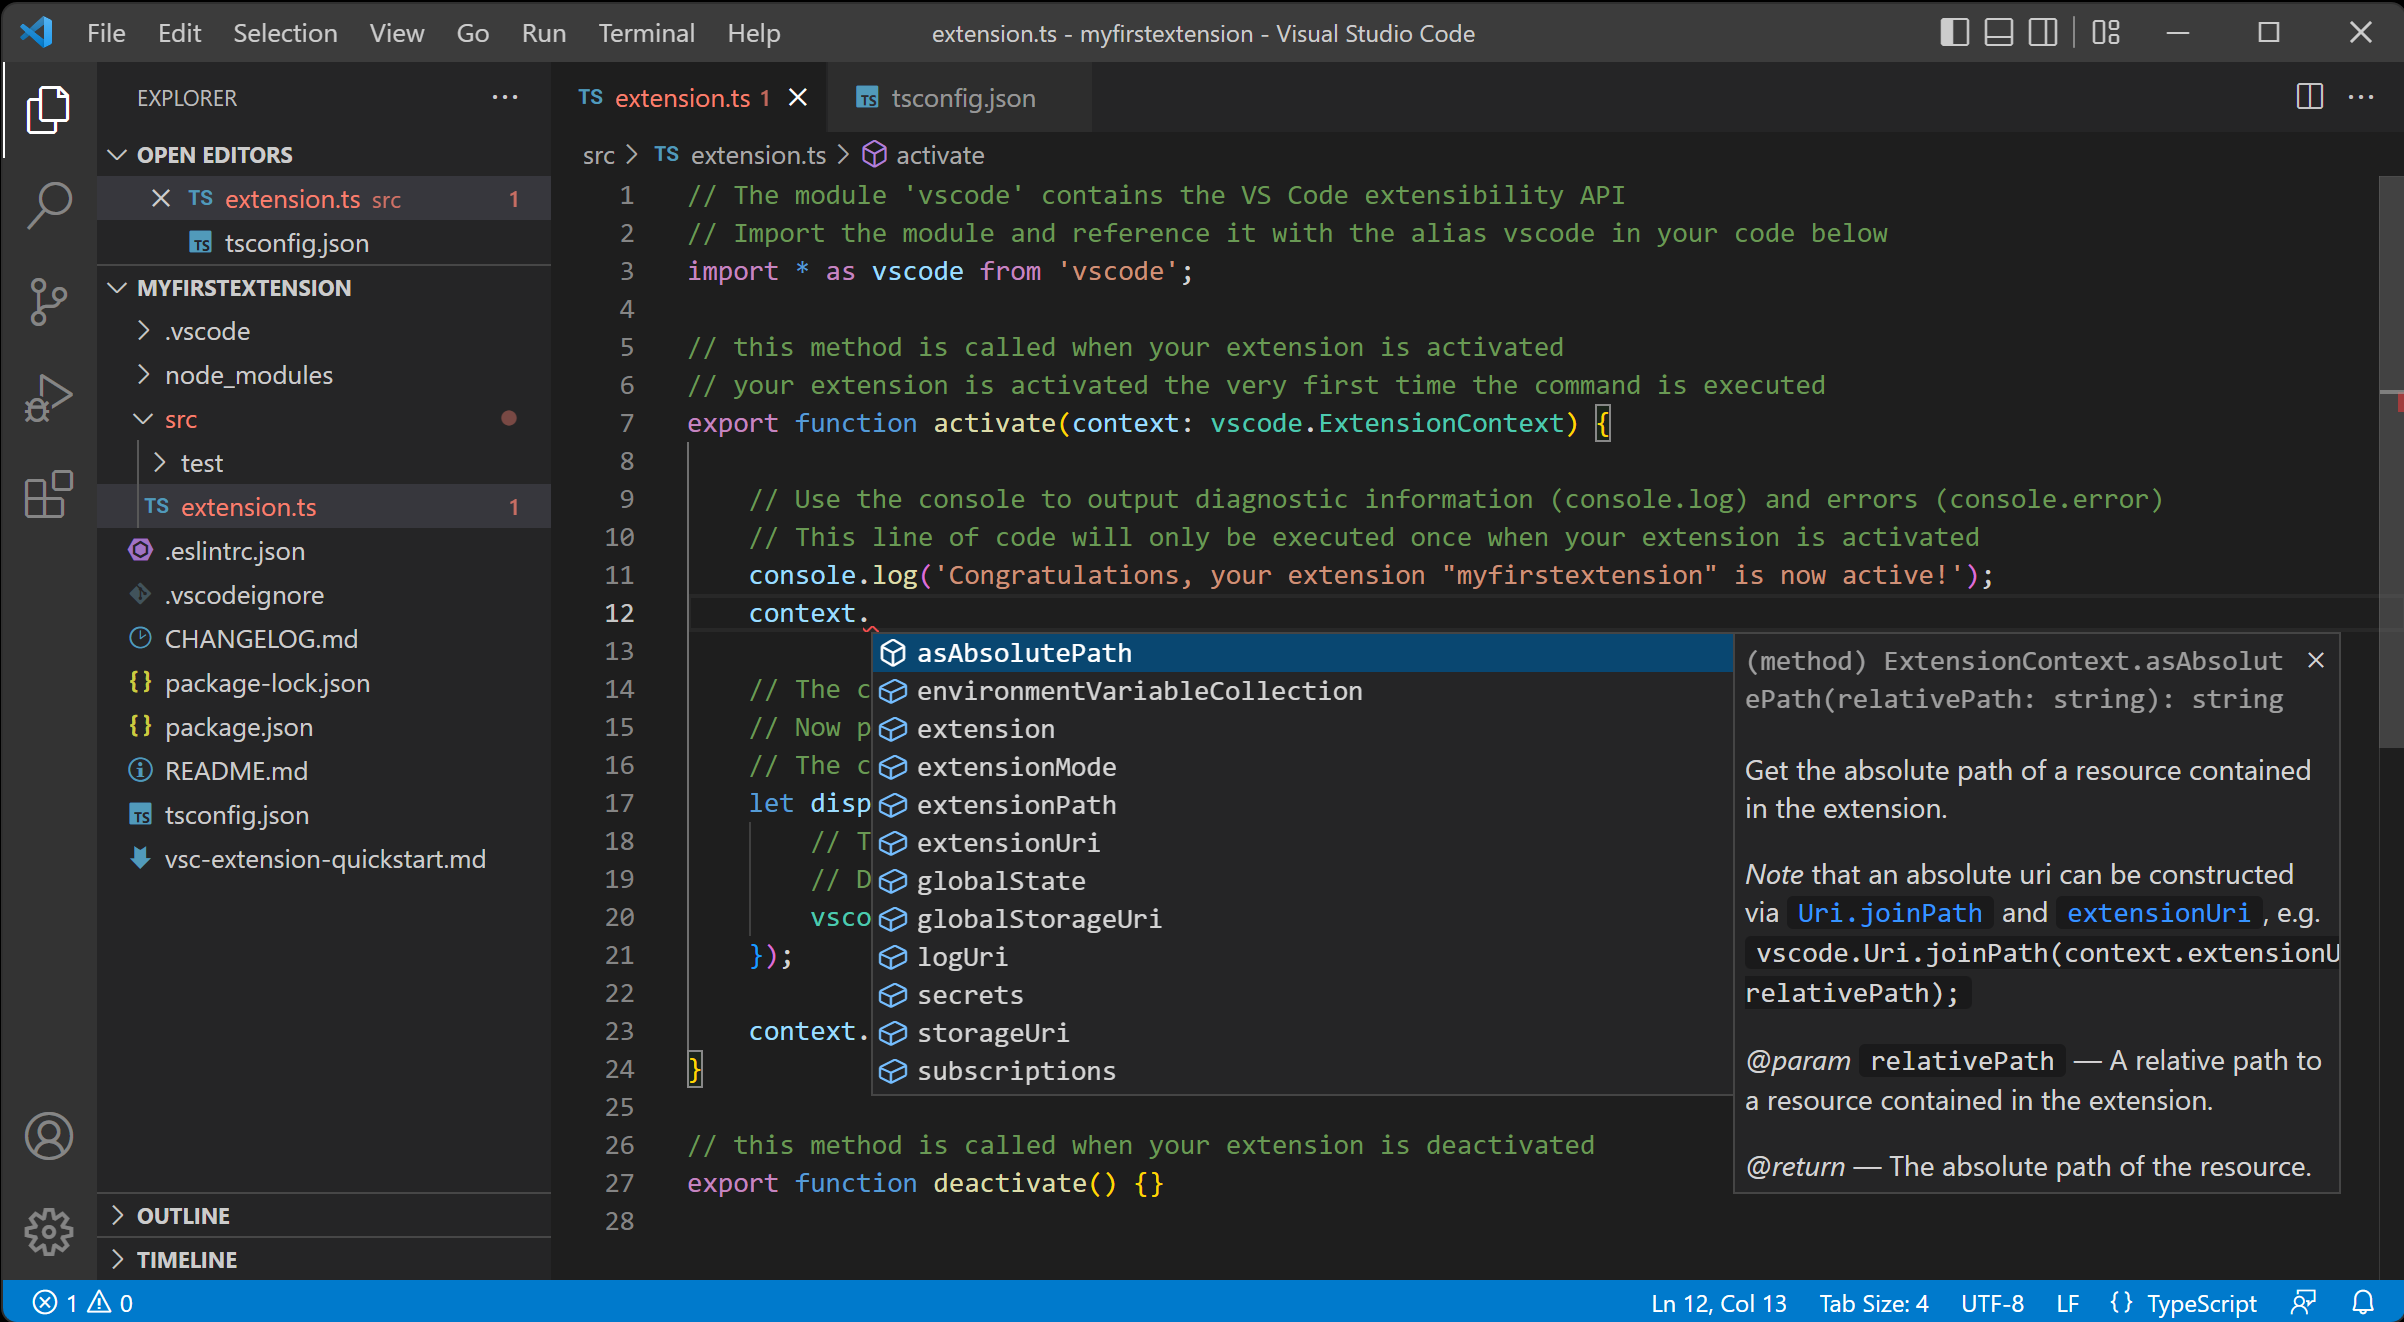
\includegraphics[scale=0.48]{pics/visualStudioCode.png}
  \caption{Ansicht Visual Studio Code}
  \label{fig:impl:vsCode}
\end{figure}

\subsection{Github [T]} \setauthor{Teresa Holzer}
% < https://github.com/features
GitHub ist ein Online-Tool, das ermöglicht, zusammen mit Teammitgliedern  an Projekten zusammenzuarbeiten. Projekte können dabei mühelos neu heruntergeladen werden, es kann auf neue Versionen aktualisiert werden, und es können Versionen mit verschiedenen Versionsnummern zusammengefügt werden. GitHub kann über das Terminal oder GitHub Desktop verwendet werden, siehe Abb. \ref{fig:impl:gitHubTerminalVSGUI}.

\begin{figure}[h t]
  \centering
  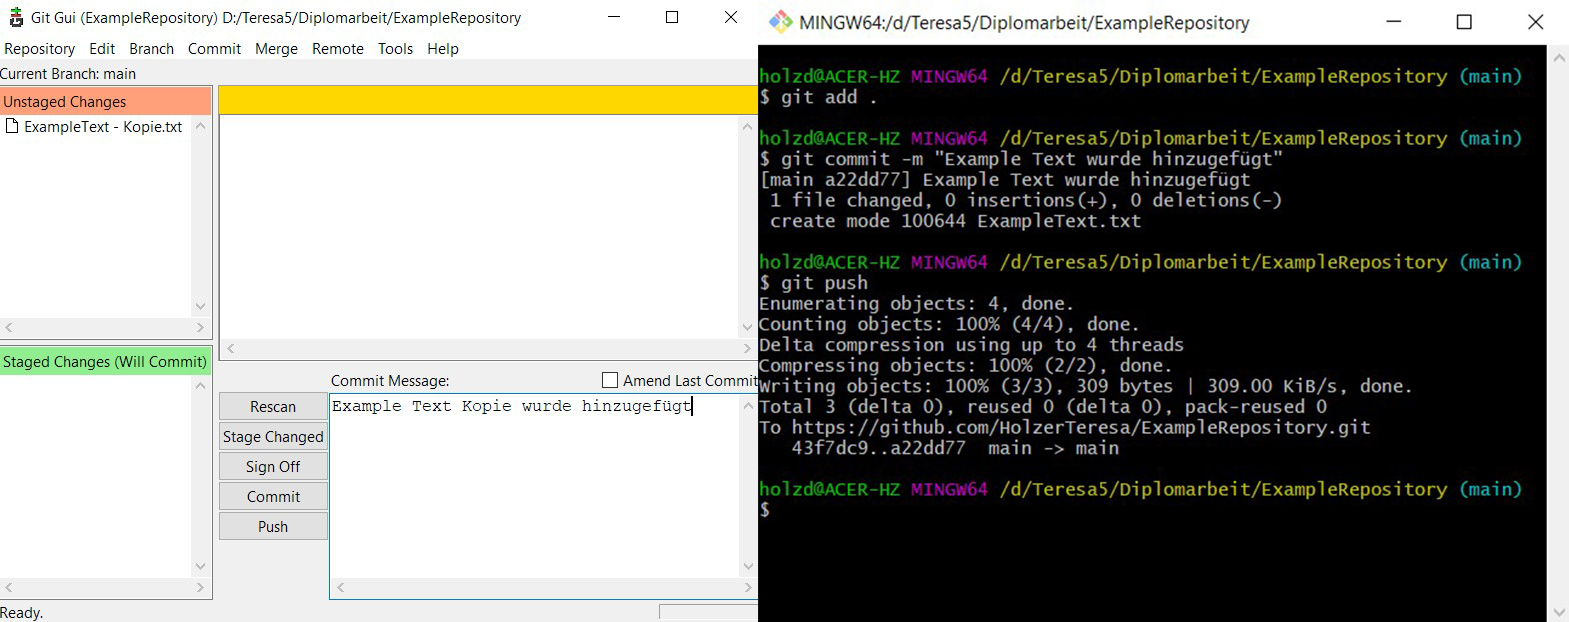
\includegraphics[scale=0.45]{pics/githubTerminalGUI.png}
  \caption{GitHub Desktop vs. Terminal}
  \label{fig:impl:gitHubTerminalVSGUI}
\end{figure}

Bei der Verwendung von GitHub können sogenannte Repositories, siehe Abb. \ref{fig:impl:githubRepository}, erstellt werden. In diese können neue Dokumente bzw. Dateien hinzugefügt werden. Ein Repository besitzt zusätzlich eine Beschreibung sowie eine Übersicht der Historie der hinzugefügten Dateien. Mithilfe dieser können vorherige Versionen wiederhergestellt bzw. gesichtet werden. Wenn also zum Beispiel die aktuelle Version eines Programms auf Discord einen Fehler enthält, kann ohne Probleme zu der vorherigen Version gewechselt werden. 



\begin{figure}[h t]
  \centering
  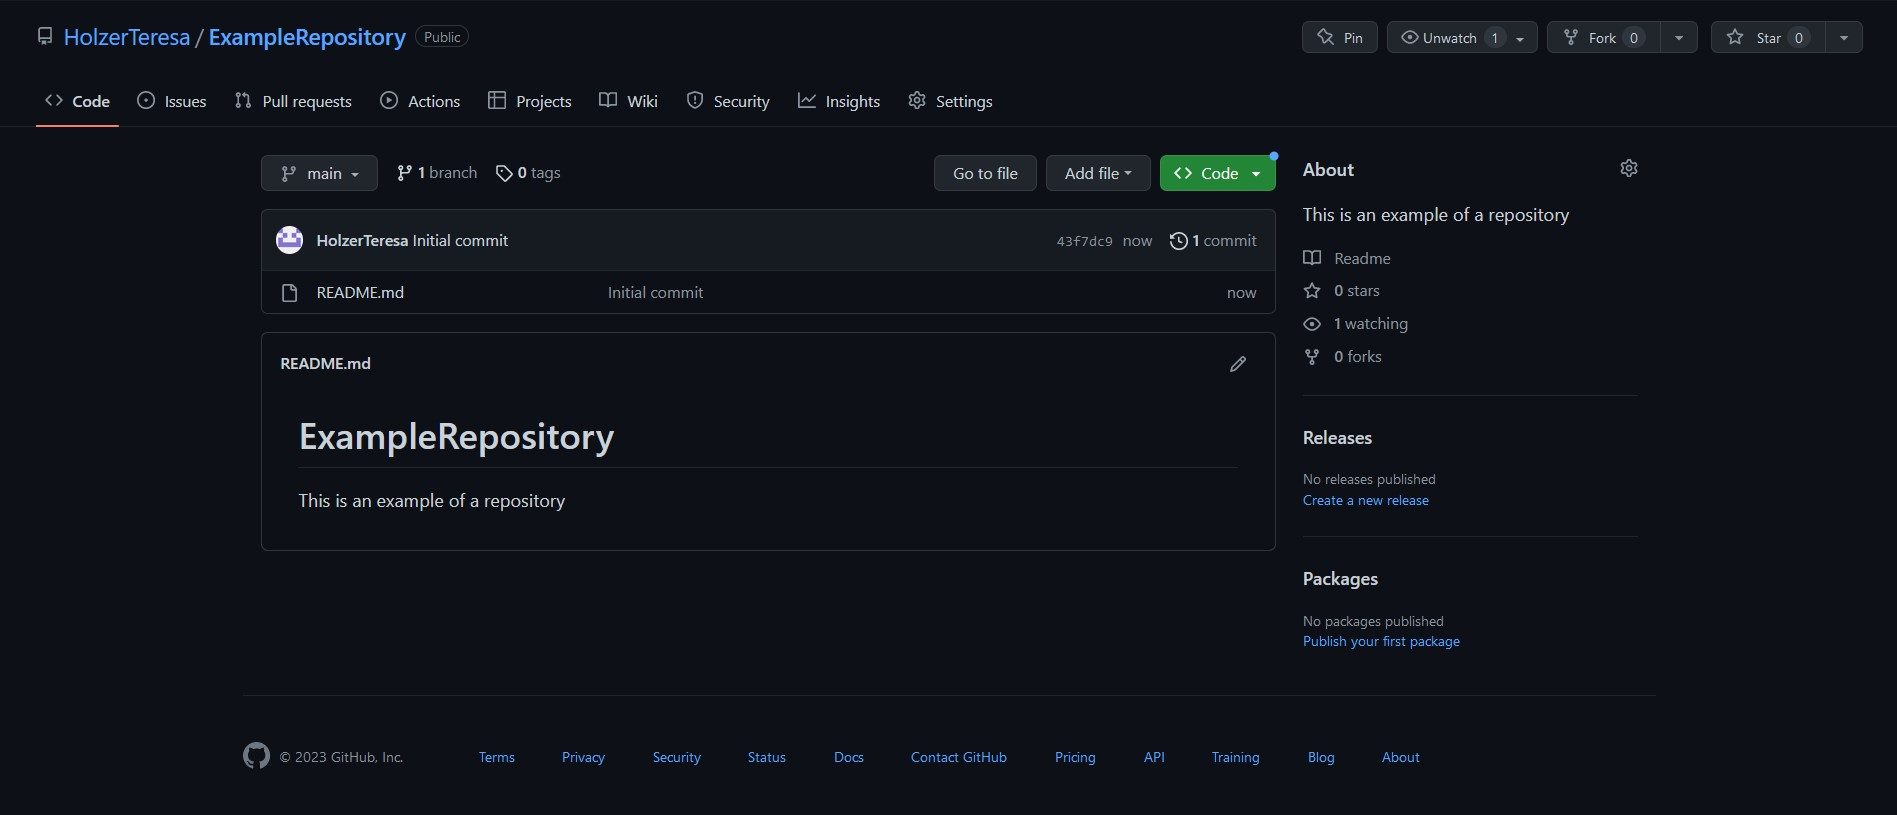
\includegraphics[scale=0.38]{pics/exampleRepository.jpg}
  \caption{Beispiel eines GitHub Repo}
  \label{fig:impl:githubRepository}
\end{figure}
